% ---------------------------------------------------------------------------- %

\section{Implementação}
\label{sec:impl}

Tendo-se apresentado as funcionalidades disponibilizadas pelo sistema \SYS, descre\-ve-se nesta secção a implementação do mesmo, primeiro delineando a sua arquitetura e depois detalhando os seus principais componentes.

% ---------------------------------------------------------------------------- %

\subsection{Arquitetura}

O sistema foi integralmente implementado na linguagem Java (versão \emph{Java SE 11}), fazendo uso das duas bibliotecas seguintes:

\begin{itemize}

    \item \emph{argparse4j}\footnote{\url{https://argparse4j.github.io/}} versão 0.8.1, utilizada para processar os argumentos da linha de comandos;
    
    \item \emph{IPAddress}\footnote{\url{https://seancfoley.github.io/IPAddress/}} versão 5.0.2, utilizada para processar \nonpt{strings} em notação CIDR, representando intervalos contíguos de endereços IPv4 ou IPv6.
    
\end{itemize}

A implementação do sistema foi divida em três camadas, a cada uma correspondendo um \nonpt{package} Java:

\begin{enumerate}

    \item \emph{Camada de comunicação fiável} (\nonpt{package} \texttt{fileshare.transport}), encapsulando a implementação do protocolo de transferência fiável de dados sobre UDP e expondo uma interface de estabelecimento de conecções para comunicação entre \nonpt{hosts};

    \item \emph{Camada de transferência de ficheiros} (\nonpt{package} \texttt{fileshare.core}), utilizando a camada anterior para implementar toda a lógica de transferência de ficheiros entre \nonpt{peers};

    \item \emph{Camada de interface de utilizador} (\nonpt{package} \texttt{fileshare.ui}), implementando a interface de linha de comandos do programa, recorrendo a serviços expostos pela camada anterior.

\end{enumerate}

As interdependências entre estes três \nonpt{packages} é ilustrada na Figura~\ref{fig:impl:packages}. O código-fonte do sistema está extensivamente documentado através de comentários Javadoc embutidos no próprio código-fonte.

\begin{figure}[ht]
  \centering
  \vspace*{.3\baselineskip}
  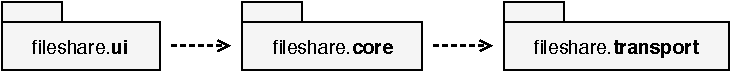
\includegraphics[scale=.9]{figures/packages.pdf}
  \caption{Dependências entre \nonpt{packages} Java da implementação do sistema.}
  \label{fig:impl:packages}
  \vspace*{.1\baselineskip}
\end{figure}

Em cada uma das subsecções seguintes, detalham-se os aspetos mais relevantes de cada uma das camadas supramencionadas, na ordem apresentada anteriormente.

% ---------------------------------------------------------------------------- %

\subsection{Camada de comunicação fiável}

A camada de comunicação fiável implementa um protocolo de comunicação sobre UDP com garantia de transmissão sem erros e de ordem. Apresenta-se aqui primeiro a interface exposta por esta camada, detalhando-se depois o funcionamento do protocolo na qual esta se baseia.

\itemizedpar{Interface disponibilizada.}

As classes que constituem a interface pública desta camada pertencem ao \nonpt{package} \texttt{fileshare.transport} e são ilustradas na Figura~\ref{fig:impl:classes-transport}, juntamente com as suas interdependências ao nível da interface.

\begin{figure}[ht]
  \centering
  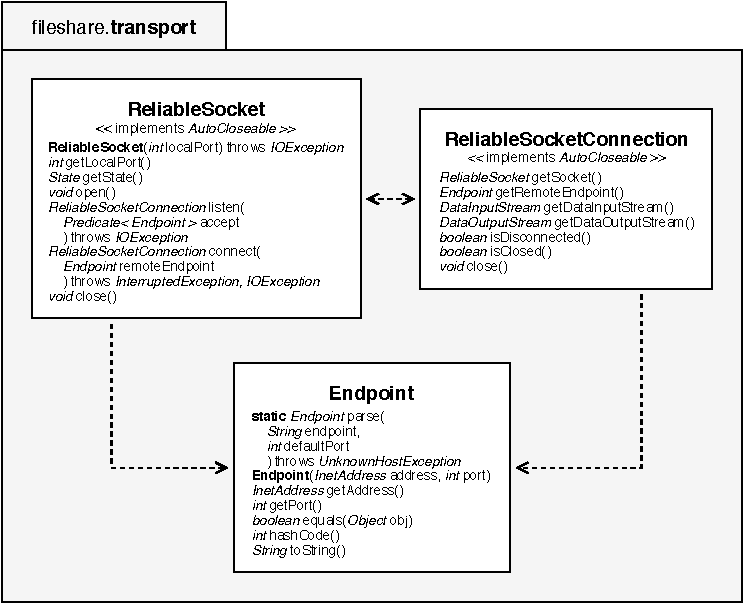
\includegraphics{figures/classes-transport.pdf}
  \caption{Classes do \emph{package} \texttt{fileshare.transport} e dependências ao nível da interface.}
  \label{fig:impl:classes-transport}
\end{figure}

A classe \texttt{Endpoint} representa um par endereço-porta, similarmente à classe \path{java.net.InetSocketAddress}. Ao contrário desta última, no entanto, a classe \texttt{Endpoint} não permite \nonpt{hostnames} não resolvidos, garantindo que erros relativos à resolução de nomes são tratados pelas camadas superiores.

A classe principal desta camada, \texttt{ReliableSocket}, gere um \nonpt{socket} UDP local, permitindo estabelecer conecções \nonpt{duplex} com outros \nonpt{sockets} similares, estas últimas sendo representadas por instâncias da classe \texttt{ReliableSocketConnection}.

O método \texttt{connect()} da classe \texttt{ReliableSocket} permite efetuar pedidos de establecimento de conecções com outros \nonpt{sockets}. O método \texttt{listen()} é utilizado para a tratar estes pedidos de conecção, permitindo também definir um predicado que determine se um dado pedido de conecção deve ser aceite ou rejeitado.

Os métodos \path{getDataInputStream()} e \path{getDataOutputStream()}, ambos da classe \path{ReliableSocketConnection}, devolvem \nonpt{streams} que podem ser utilizadas para se receber e enviar dados através da conecção respetiva. O método \path{close()} termina a conecção.

Para mais informações sobre a interface exposta por esta camada, remete-se o leitor para a documentação \nonpt{Javadoc} embutida no código-fonte.

\itemizedpar{Protocolo de comunicação fiável.}

A camada de comunicação fiável permite estabelecer canais \nonpt{duplex} de comunicação orientados à conecção, com garantia de transmissão sem erros, sem dados duplicados e ordenada. Todas as interações entre os \nonpt{sockets} descritos acima são, internamente, realizadas através de \nonpt{packets}, os quais podem ser de vários tipos, cada um tendo o seu formato específico. Estes tipos, significados correspondentes e formatos são especificados na Tabela~\ref{tbl:impl:tipos-packets}.

\begin{table}[ht]
  \centering
  \setlength{\tabcolsep}{6.5pt}
  \renewcommand{\arraystretch}{1.3}
  \begin{tabularx}{\textwidth}{|l|X|l|}
  
    \hline
    \multicolumn{1}{|c|}{\textbf{Tipo}} &
    \multicolumn{1}{c|}{\textbf{Descrição}} &
    \multicolumn{1}{c|}{\textbf{Formato}}
    \\ \hline
    
    \texttt{CONN}
     & \multirow[t]{3}{=}{Pedido de estabelecimento de conecção}
       & 4 bytes: Checksum \\
     & & 1 byte: Identificador do tipo de pacote (= 0) \\
     & & 2 bytes: Identificador local da conecção \\
    \hline
    
    \texttt{CONN-ACCEPT}
     & \multirow[t]{3}{=}{Notificação da aceitação de um pedido de conecção}
       & 4 bytes: Checksum \\
     & & 1 byte: Identificador do tipo de pacote (= 1) \\
     & & 2 bytes: Identificador remoto da conecção \\
     & & 2 bytes: Identificador local da conecção \\
    \hline

    \texttt{CONN-REJECT}
     & \multirow[t]{3}{=}{Notificação da rejeição de um pedido de conecção}
       & 4 bytes: Checksum \\
     & & 1 byte: Identificador do tipo de pacote (= 2) \\
     & & 2 bytes: Identificador remoto da conecção \\
    \hline
    
    \texttt{DATA}
     & \multirow[t]{3}{=}{Envio de dados}
       & 4 bytes: Checksum \\
     & & 1 byte: Identificador do tipo de pacote (= 3) \\
     & & 2 bytes: Identificador local da conecção \\
     & & 8 bytes: Posição dos dados na \emph{stream} \\
     & & Entre 1 e 1415 bytes: Dados (\emph{payload}) \\
    \hline
    
    \texttt{DATA-ACK}
     & \multirow[t]{3}{=}{Confirmação da receção de dados}
       & 4 bytes: Checksum \\
     & & 1 byte: Identificador do tipo de pacote (= 4) \\
     & & 2 bytes: Identificador local da conecção \\
     & & 8 bytes: Posição na \emph{stream} tal que todos os \\
     & & \hfill dados anteriores tenham sido recebidos \\
    \hline
    
    \texttt{DISC}
     & \multirow[t]{3}{=}{Notificação do término da conecção}
       & 4 bytes: Checksum \\
     & & 1 byte: Identificador do tipo de pacote (= 5) \\
     & & 2 bytes: Identificador local da conecção \\
    \hline
    
    \texttt{DISC-ACK}
     & \multirow[t]{3}{=}{Confirmação da receção da notificação do término da conecção}
       & 4 bytes: Checksum \\
     & & 1 byte: Identificador do tipo de pacote (= 6) \\
     & & 2 bytes: Identificador local da conecção \\
    \hline
    
  \end{tabularx}
  \caption{Tipos de \nonpt{packets} trocados pelo protocolo de comunicação fiável.}
  \label{tbl:impl:tipos-packets}
\end{table}

A descrição que se segue faz referência a vários valores não especificados, tais como \nonpt{timeouts} e números máximos de retransmissões. Estes valores estão definidos na classe \texttt{Config} do \nonpt{package} \texttt{fileshare.transport}.

Os primeiros 5 bytes de todos os \nonpt{packets} seguem o mesmo formato: 4 bytes para um \nonpt{checksum} e 1 byte para identificar o tipo de \nonpt{packet}. O \nonpt{checksum} é computado por quem envia o \nonpt{packet}, com base no conteúdo do mesmo, e é recomputado e comparado pelo destinatário. Se o \nonpt{checksum} recebido no \nonpt{packet} tiver um valor distinto do computado pelo recipiente, o \nonpt{packet} é simplesmente descartado.

Por forma a se estabelecer uma conecção, é enviado um \nonpt{packet} do tipo \texttt{CONN}. Ao receber um destes \nonpt{packets}, o recipiente responde com um outro \nonpt{packet} do tipo \texttt{CONN-ACCEPT} ou \texttt{CONN-REJECT}, aceitando ou rejeitando a conecção, respetivamente. Se o \nonpt{packet} \texttt{CONN} não obtiver resposta, este é reenviado (após um determinado intervalo de tempo). Se após um certo número de retransmissões não existir resposta, é reportado um erro à camada superior.

Após se estabelecer uma conecção, ambos os lados da conecção podem enviar dados através de \texttt{packets} do tipo \texttt{DATA}. O recipiente deve depois enviar um \nonpt{packet} \texttt{DATA-ACK} por forma a reconhecer a receção dos dados. Se não for recebido um \nonpt{packet} \texttt{DATA-ACK}, os dados são retransmitidos. Resumidamente, é seguida uma abordagem \emph{Go-Back-N}, não existem \nonpt{acknowledgments} negativos e os \nonpt{acknowledgments} são cumulativos e expressos como \nonpt{offsets} em bytes correspondentes aos dados recebidos desde que a conecção foi estabelecida.

Ao terminar uma conecção é enviado um \nonpt{packet} \texttt{DISC}, aguardando-se depois uma resposta na forma de um \nonpt{packet} \texttt{DISC-ACK}. O \nonpt{packet} \texttt{DISC} é retransmitido se não houver resposta, até um determinado número máximo de retransmissões, após o qual a conecção é considerada, de qualquer forma, terminada.

Se um dos lados da conecção morrer, isto é detetado pela ausência de respostas \texttt{DATA-ACK} a dados enviados, e a conecção é dada como terminada.

% ---------------------------------------------------------------------------- %

\subsection{Camada de transferência de ficheiros}

A camada de transferência de ficheiros implementa, com recurso à camada de comunicação fiável previamente descrita, o protocolo \nonpt{peer-to-peer} de transferência de ficheiros disponibilizado pelo sistema \SYS. De seguida apresenta-se a interface exposta por esta camada, descrevendo-se também os protocolos de comunicação entre \nonpt{peers} para a execução de transferências de ficheiros.

\itemizedpar{Interface disponibilizada.}

As classes que constituem a interface pública da camada de transferência de ficheiros, todas pertencentes ao \nonpt{package} \path{fileshare.core}, são ilustradas na Figura~\ref{fig:impl:classes-core} juntamente com as suas interdependências ao nível da interface.

\begin{figure}[p]
  \centering
  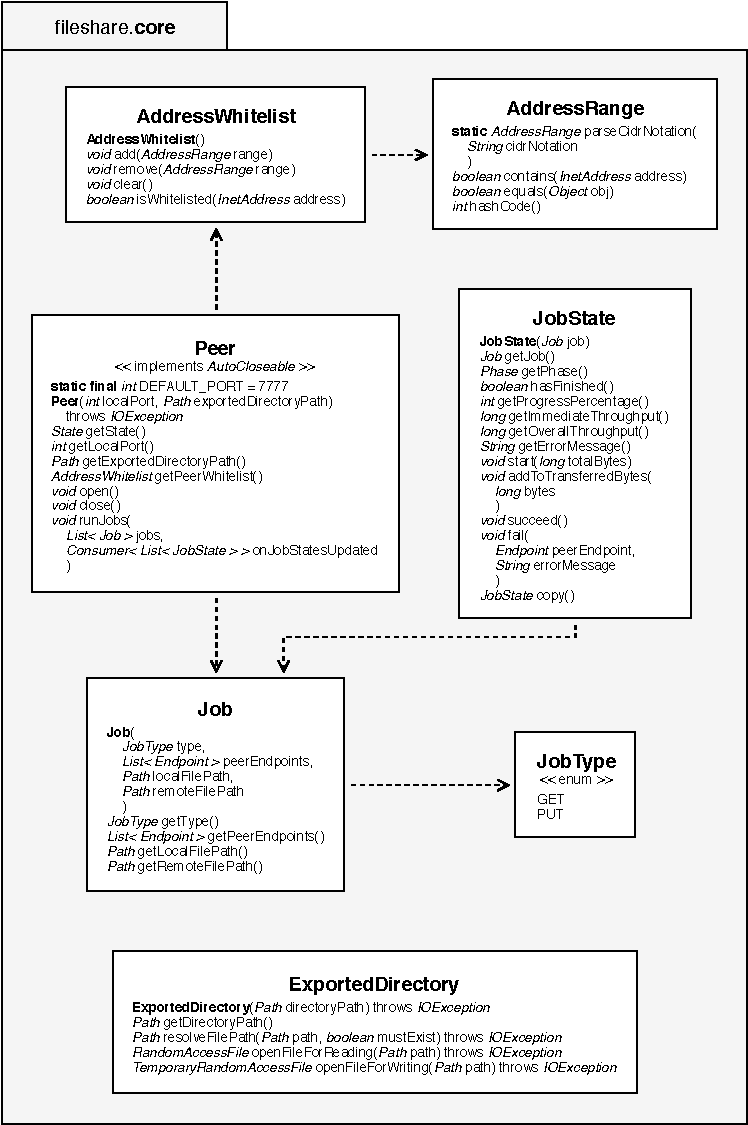
\includegraphics{figures/classes-core.pdf}
  \caption{Classes do \emph{package} \texttt{fileshare.core} e dependências ao nível da interface.}
  \label{fig:impl:classes-core}
\end{figure}

A classe \texttt{Peer} gere um \nonpt{peer} local no sistema \SYS, sendo então a classe central desta camada. A sua interface permite gerir a \nonpt{whitelist} de endereços de \nonpt{peers}, descrita previamente, e, através do método \texttt{runJobs()}, iniciar a execução de transferências de ficheiros --- aqui denominadas de \emph{jobs} --- com outros \nonpt{peers}. Esta classe serve também, em segundo plano, pedidos de transferência de ficheiros realizados por outros \nonpt{peers}.

Brevemente, as restantes classes e enumerações têm as seguintes responsabilidades:

\begin{itemize}
    \item \texttt{AddressRange} -- representa um intervalo contíguo de endereços IPv4 ou IPv6;
    \item \texttt{AddressWhitelist} -- utilizada para representar a \nonpt{whitelist} de endereos de \nonpt{peers};
    \item \texttt{ExportedDirectory} -- gere a sub-árvore do sistema de ficheiros exportada pelo \nonpt{peer};
    \item \texttt{JobType} -- define os dois tipos de transferência: \nonpt{download} (\texttt{GET}) e \nonpt{upload} (\texttt{PUT});
    \item \texttt{Job} -- define uma transferência de um ficheiro, em qualquer direção e envolvendo qualquer número de \nonpt{peers} remotos;
    \item \texttt{JobState} -- representa o estado de um \nonpt{job} que está a decorrer.
\end{itemize}

Para mais informações sobre a interface exposta por esta camada, remete-se o leitor para a documentação \nonpt{Javadoc} embutida no código-fonte.

\itemizedpar{Protocolo de transferência de ficheiros.}

Para executar um \nonpt{job}, o \nonpt{peer} estabelece conecções com todos os outros \nonpt{peers} envolvidos na transferência e segue, depois, um protocolo de comunicação específico à direção da transferência.

Os protocolos utilizados em transferências dos tipos \emph{get} e \emph{put} são delineados nas Tabelas~\ref{tbl:impl:protocolo-get} e~\ref{tbl:impl:protocolo-put}, respetivamente, onde o \emph{cliente} corresponde ao \nonpt{peer} que requeriu a transferência e o \emph{servidor} corresponde ao \nonpt{peer} restante (caso exista mais de um \nonpt{peer} remoto, o protocolo é seguido para cada um deles). Explicita-se que estas tabelas não são uma especificação completa do protocolo, em particular não apresentando todos os casos de erro, destinando-se apenas a ilustrar a implementação do mesmo.

\begin{table}[p]
    \centering
    \setlength{\tabcolsep}{6.5pt}
    \renewcommand{\arraystretch}{1.15}
    \begin{tabularx}{\textwidth}{|p{2cm}|X|X|}
        \cline{2-3}
        \multicolumn{1}{l|}{} & \multicolumn{1}{c|}{\textbf{Cliente}} & \multicolumn{1}{c|}{\textbf{Servidor}} \\
        \hline \multirow[t]{5}{=}{Comportamento normal}
         & \verb|writeByte(0)| (tipo de \emph{job}) & \\
         & \verb|writeUTF(path_file_servidor)| & \\
         & \verb|flush()| & \\
         & & \verb|readByte()| (= 0) \\
         & & \verb|path_file_servidor = readUTF()| \\
         & & [se erro, ir para \emph{caso de erro 1}] \\
         & & \verb|writeLong(tamanho_file)| \\
         & & \verb|flush()| \\
         & \verb|tamanho_file = readLong()| & \\
         & [se erro, ir para \emph{caso de erro 2}] & \\
         & \verb|writeLong(offset_segmento)| & \\
         & \verb|writeLong(tamanho_segmento)| & \\
         & \verb|flush()| & \\
         & & \verb|offset_segmento = readLong()| \\
         & & \verb|tamanho_segmento = readLong()| \\
         & & escreve conteúdo do segmento \\
         & & \verb|flush()| \\
         & & \verb|close()| \\
         & lê e armazena conteúdo do segmento & \\
         & \verb|close()| & \\
        \hline \multirow[t]{5}{=}{Caso de erro 1 (\emph{e.g.}, ficheiro não existe no servidor)}
         & & \verb|writeLong(-1)| \\
         & & \verb|writeUTF(mensagem_erro)| \\
         & & \verb|flush()| \\
         & & \verb|close()| \\
         & \verb|readLong()| (= -1) & \\
         & \verb|mensagem_erro = readUTF()| & \\
         & reporta erro & \\
         & \verb|close()| & \\
        \hline \multirow[t]{5}{=}{Caso de erro 2 (\emph{e.g.}, tamanhos distintos entre servidores)}
         & reporta erro & \\
         & \verb|close()| & \\
         & & deteta \emph{end-of-file} \\
         & & \verb|close()| \\
        \hline
    \end{tabularx}
    \caption{Protocolo de comunicação entre dois \emph{peers}, ao nível da camada de transferência de ficheiros, para execução de um \emph{job} do tipo \emph{get}.}
    \label{tbl:impl:protocolo-get}
\end{table}

\begin{table}[p]
    \centering
    \setlength{\tabcolsep}{6.5pt}
    \renewcommand{\arraystretch}{1.15}
    \begin{tabularx}{\textwidth}{|p{2cm}|X|X|}
        \cline{2-3}
        \multicolumn{1}{l|}{} & \multicolumn{1}{c|}{\textbf{Cliente}} & \multicolumn{1}{c|}{\textbf{Servidor}} \\
        \hline \multirow[t]{5}{=}{Comportamento normal}
         & \verb|writeByte(1)| (tipo de \emph{job}) & \\
         & \verb|writeUTF(path_file_servidor)| & \\
         & \verb|writeLong(tamanho_file)| & \\
         & \verb|flush()| & \\
         & & \verb|readByte()| (= 1) \\
         & & \verb|path_file_servidor = readUTF()| \\
         & & \verb|tamanho_file = readLong()| \\
         & & [se erro, ir para \emph{caso de erro 1}] \\
         & & \verb|writeUTF("")| \\
         & & \verb|flush()| \\
         & \verb|readUTF()| (= \verb|""|) & \\
         & escreve conteúdo do ficheiro & \\
         & \verb|flush()| & \\
         & & lê e armazena conteúdo do ficheiro \\
         & & [se erro, ir para \emph{caso de erro 2}] \\
         & & \verb|writeUTF("")| \\
         & & \verb|flush()| \\
         & & \verb|close()| \\
         & \verb|readUTF()| (= \verb|""|) & \\
         & \verb|close()| & \\
        \hline \multirow[t]{5}{=}{Caso de erro 1 (\emph{e.g.}, ficheiro está em utilização)}
         & & \verb|writeUTF(mensagem_erro)| \\
         & & \verb|flush()| \\
         & & \verb|close()| \\
         & \verb|mensagem_erro = readUTF()| & \\
         & \verb|close()| & \\
         & reporta erro & \\
        \hline \multirow[t]{5}{=}{Caso de erro 2 (\emph{e.g.}, erro ao escrever ficheiro)}
         & & \verb|writeUTF(mensagem_erro)| \\
         & & \verb|flush()| \\
         & & \verb|close()| \\
         & \verb|mensagem_erro = readUTF()| & \\
         & \verb|close()| & \\
         & reporta erro & \\
        \hline
    \end{tabularx}
    \caption{Protocolo de comunicação entre dois \emph{peers}, ao nível da camada de transferência de ficheiros, para execução de um \emph{job} do tipo \emph{put}.}
    \label{tbl:impl:protocolo-put}
\end{table}

% ---------------------------------------------------------------------------- %

\subsection{Camada de interface de utilizador}

Por fim, a camada de interface de utilizador implementa a interface de linha de comandos disponibilizada pelo comando \path{fileshare}. Para efeitos de referência, as classes que implementam esta camada são ilustradas na Figura~\ref{fig:impl:classes-ui}. No entanto, considera-se que a descrição detalhada desta camada está fora do âmbito do presente relatório.

Como tal, para mais informações sobre a implementação desta camada, remete-se o leitor para a documentação \emph{Javadoc} embutida no código-fonte.

\begin{figure}[ht]
  \centering
  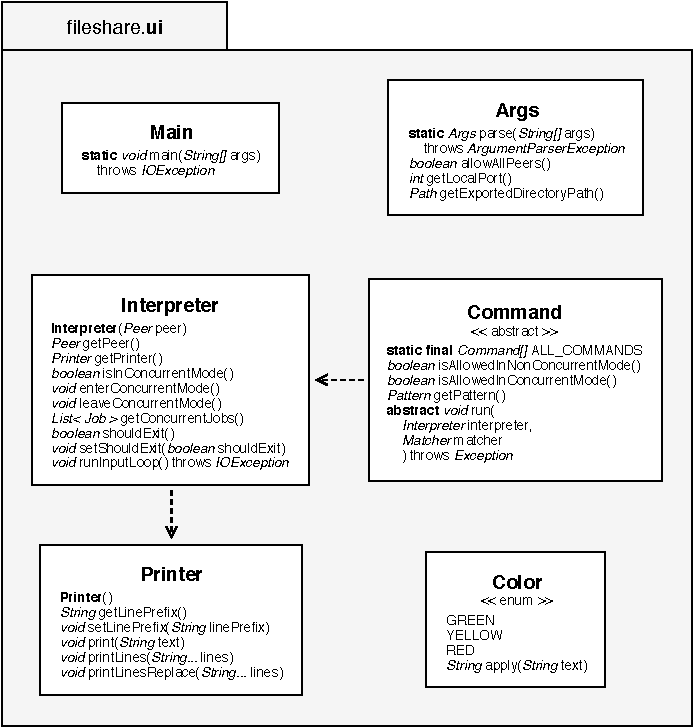
\includegraphics{figures/classes-ui.pdf}
  \caption{Classes do \emph{package} \texttt{fileshare.ui} e dependências ao nível da interface.}
  \label{fig:impl:classes-ui}
\end{figure}

% ---------------------------------------------------------------------------- %
